\documentclass[a4paper,12pt]{article} 
\usepackage{tikz}
\usepackage{xeCJK}
\usetikzlibrary{petri}


\begin{document}

\begin{tikzpicture}
  \node[place,label=above:$p_1$] (p1) {};
%  \node[place,label=above;$p_2\ge1$,right=of p1] (p2) {};
  \node[place,label=below:$p_2$, right=5cm,tokens=2 ] (p2) {};
\end{tikzpicture}




\newpage
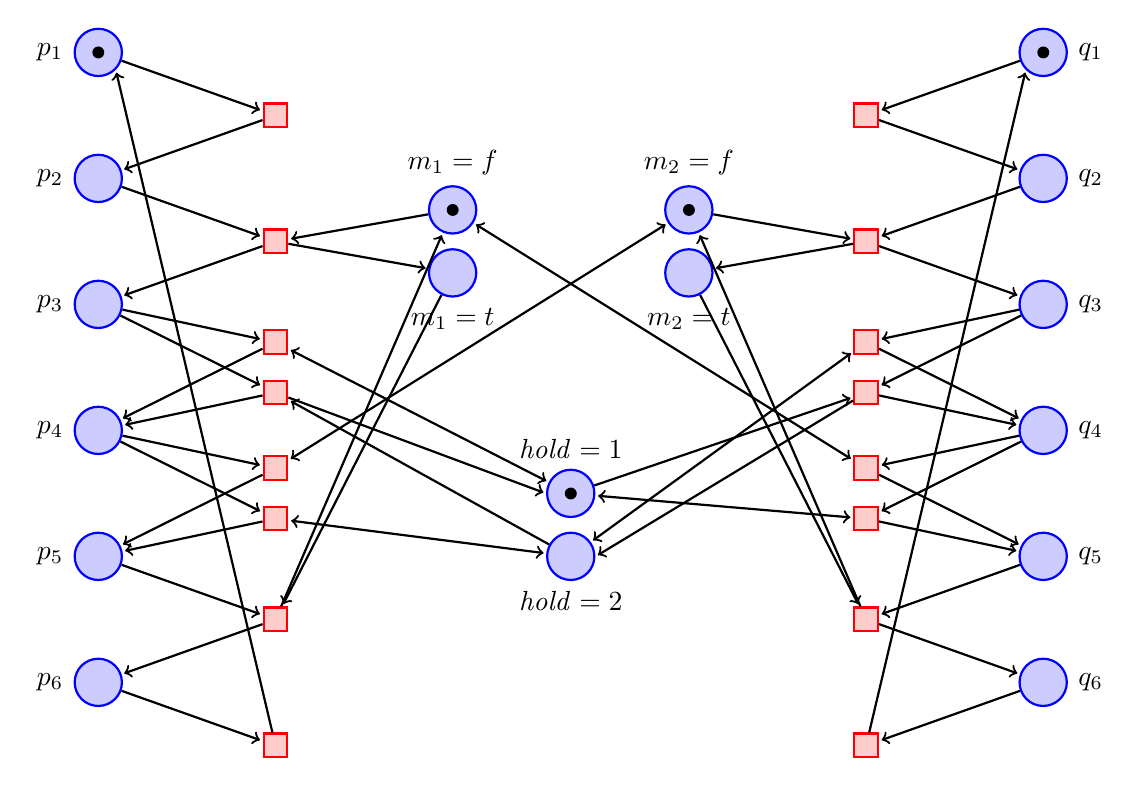
\begin{tikzpicture}[yscale=-1.6,xscale=1.5,thick,
every transition/.style={draw=red,fill=red!20,minimum size=3mm},
every place/.style={draw=blue,fill=blue!20,minimum size=6mm}]
\foreach \i in {1,...,6} {
\node[place,label=left:$p_\i$] (p\i) at (0,\i) {};
\node[place,label=right:$q_\i$] (q\i) at (8,\i) {};
}
\foreach \name/\var/\vala/\valb/\height/\x in
{m1/m_1/f/t/2.25/3,m2/m_2/f/t/2.25/5,h/\mathit{hold}/1/2/4.5/4} {
\node[place,label=above:{$\var = \vala$}] (\name\vala) at (\x,\height) {};
\node[place,yshift=-8mm,label=below:{$\var = \valb$}] (\name\valb) at (\x,\height) {};
}
\node[token] at (p1) {};
 \node[token] at (q1) {};
\node[token] at (m1f) {}; \node[token] at (m2f) {};
\node[token] at (h1) {};
\node[transition] at (1.5,1.5) {}
 edge
 [pre] (p1) edge [post] (p2);
\node[transition] at (1.5,2.5) {}
 edge
 [pre] (p2) edge[pre]
 (m1f)
edge
 [post](p3) edge[post] (m1t);
\node[transition] at (1.5,3.3) {}
 edge
 [pre] (p3) edge [post] (p4)
edge
 [pre and post] (h1);
\node[transition] at (1.5,3.7) {}
 edge
 [pre] (p3) edge [pre] (h2)
edge
 [post] (p4) edge [post] (h1.west);
\node[transition] at (1.5,4.3) {}
 edge
 [pre] (p4) edge [post] (p5)
edge
 [pre and post] (m2f);
\node[transition] at (1.5,4.7) {}
 edge
 [pre] (p4) edge [post] (p5)
edge
 [pre and post] (h2);
\node[transition] at (1.5,5.5) {}
 edge
 [pre] (p5) edge [pre] (m1t)
edge
 [post] (p6) edge [post] (m1f);
\node[transition] at (1.5,6.5) {}
 edge
 [pre] (p6) edge [post] (p1.south east);
\node[transition] at (6.5,1.5) {}
 edge
 [pre] (q1) edge [post] (q2);
\node[transition] at (6.5,2.5) {}
 edge
 [pre] (q2) edge [pre] (m2f)
edge
 [post] (q3) edge [post] (m2t);
\node[transition] at (6.5,3.3) {}
 edge
 [pre] (q3) edge [post] (q4)
edge
 [pre and post] (h2);
\node[transition] at (6.5,3.7) {}
 edge
 [pre] (q3) edge [pre] (h1)
edge
 [post] (q4) edge [post] (h2.east);
\node[transition] at (6.5,4.3) {}
 edge
 [pre] (q4) edge [post] (q5)
edge
 [pre and post] (m1f);
\node[transition] at (6.5,4.7) {}
 edge
 [pre] (q4) edge [post] (q5)
edge
 [pre and post] (h1);
\node[transition] at (6.5,5.5) {}
 edge
 [pre] (q5) edge [pre] (m2t)
edge
 [post] (q6) edge [post] (m2f);
\node[transition] at (6.5,6.5) {}
 edge
 [pre] (q6) edge [post] (q1.south west);
\end{tikzpicture}


\end{document}
